\documentclass[a4paper]{article}

%% Language and font encodings
\usepackage[french]{babel}
\usepackage[utf8x]{inputenc}
\usepackage[T1]{fontenc}
\usepackage{amssymb}

%% Sets page size and margins
\usepackage[a4paper,top=3cm,bottom=2cm,left=3cm,right=3cm,marginparwidth=1.75cm]{geometry}

%% Useful packages
\usepackage{amsmath}
\usepackage{graphicx}
\usepackage[colorinlistoftodos]{todonotes}
\usepackage[colorlinks=true, allcolors=blue]{hyperref}

\title{Projet de vérification formelle}
\author{Alexandre PINON, Souhaib ATTAIKI}
\date{Feb 2018}

\begin{document}
\maketitle

\begin{abstract}

\href{https://github.com/souhaibattaiki/ivf-program-verifier}{Lien GitHub}

Dans le cadre de ce projet, nous avons choisi se heurter à la difficulté de construire un arbre abstrait de syntaxe (ou AST) complet sans avoir recours à de librairies externes sur la base d'une syntaxe que nous définissons nous-même. 

Nous utilisons l'AST pour l'interprétation du programme et en particulier pour la génération d'un graphe de contrôle (CFG). 

\textbf{Le temps} que nous avons pris pour ces deux étapes a \textbf{surpassé toutes nos prévisions} et nous n'avons ainsi \textbf{pas pu finir d'implémenter tous les critères} de test et leur génération...

\textbf{Remarque :}\textit{ Le code source étant en anglais, nous utiliserons régulièrement l’anglicisme dans le rapport pour faire référence aux classes et aux méthodes. Ainsi par exemple $interpreter$ renvoie à la classe $Interpreter$ qui constitue en réalité l'interpréteur du langage.}
\end{abstract}

\tableofcontents

\newpage

\section{Interprétation du langage WHILE}

Nous introduisons dans cette section le langage WHILE tel que nous l'avons défini et qu'il est implémenté. Par la suite, nous expliquons comment nous avons développé un $lexer$, $parser$ et $interpreter$ pour le langage. En pratique, l'interprétation du langage se base sur un arbre de syntaxe abstrait (AST) que nous avons développé entièrement après avoir défini la syntaxe en prenant en compte tous les éléments de grammaire. 

\subsection{Syntaxe} 

La grammaire du langage est définie comme suivant:
\begin{align*}
c & := l : skip & (1) \\ 
  & | \;  l : X := a & (2)\\
  & | \;  l : (c;c)  & (3)\\
  & | \;  l : if \; l : b \; then \; c \; else \; c & (4) \\ 
  & | \; l : while \; l : b \; do \;c & (5)
 \end{align*}

En terme de syntaxe, nous choisissons d'écrire (1) comme une absence d'instruction. Chaque instruction (c) est séparée par un point-virgule (;) comme dans (3). Les blocs $if$ et $while$ commencent par \textit{IF} (4) et \textit{WHILE} (5). Les décisions (limitées à une condition dans notre projet) sont évaluées entre parenthèses. Les blocs d'instruction selon qu'une décision est vraie ou fausse sont indiquées par des accolades \{ | \}. Nous avons également rajouté des commentaires encadrés de "\#". Les labels composés d'un entier suivi immédiatement de deux-points. Enfin, les assignations sont marquées d'un "=" (2). 

Pour construire un AST complet sur tout le programme, nous avons besoin de décrire la structure du langage en blocs de plus en plus petits, chaque bloc devant être simple à comprendre et parfaitement délimité. Cette description permet ensuite de d'interpréter le programme en remontant les feuilles de l'AST (identifiant une variable ou un entier) jusqu'à la racine (identifiant le début du programme). 

La syntaxe complète (et difficile) du programme est la suivante: 
\begin{verbatim}
        program :  compounds EOF
        compounds : compound | compounds
        compound : if_block | while_block | block
        if_block : IF(  cond_block  )  {  compound  }
                    | IF(  cond_block  )  { compound }  ELSE  {  compound  }
        while_block : WHILE(  cond_block  )  {  compound  }
        cond_block : label condition
        block : label statement_list
        condition : variable SUPERIOR|INFERIOR|EQUAL expr
        variable_declaration : ID (COMMA ID)* COLON type_spec
        statement_list : statement
                       | statement SEMI statement_list
        statement : statement_list
                  | assignment_statement
                  | empty
        assignment_statement : variable ASSIGN expr
        empty :
        expr : term ((PLUS | MINUS) term)*
        term : factor ((MUL | INTEGER_DIV | FLOAT_DIV) factor)*
        factor : PLUS factor
               | MINUS factor
               | INTEGER_CONST
               | LPAREN expr RPAREN
               | variable
        variable: ID
\end{verbatim}
La syntaxe permet d'évaluer des programmes ayant des sous-programmes dans les boucles \textit{IF} et \textit{WHILE}. 
Les éléments structurels de la syntaxe les plus importants sont les suivants: 
\begin{itemize}
\item \textit{block}: un label et une suite d'assignations (statement\_list) 
\item $condblock$: un label et une condition
\item $compound$: soit un bloc \textit{IF} soit \textit{WHILE} soit un simple $block$. Il est nécessaire de faire la différence car les blocs \textit{IF} et \textit{WHILE} sont connectés à des blocs qui peuvent eux-mêmes contenir des sous-programmes (liste de $compound$) et qui ne sont pas nécessairement visités. 
\item \textit{expr}, \textit{term}, \textit{factor}, \textit{variable}:  une syntaxe pour évaluer des expressions en tenant compte de la précédence (priorité) des opérations de multiplication et de divisions, avec des parenthèses. La syntaxe est emprunté à l'article\cite{1}.
\end{itemize}

\subsection{$Lexer$}

A partir de la grammaire, nous avons défini une syntaxe pour décomposer tout programme en éléments simples de manière récursive. Le $lexer$ est l'élément du module développé permettant de reconnaître les $tokens$ du programme. 

\subsubsection{Liens entre $lexer$, $parser$ et $interpreter$}

Le rôle du $lexer$ est de lire le code source et de reconnaître les différents éléments syntaxiques (dits $Tokens$) pour le $parser$. Le $parser$ retourne un arbre de syntaxe qui peut ensuite être interprété par l’interpréteur. L'interpréteur évalue chaque définition et chaque décision jusqu'à la fin du programme par visite de l'arbre en profondeur. 

En plus, nous définissions des classes pour représenter les différents types de nœuds de l'AST ($program$, $block$, $label$, $BinOp$, etc...). 

\subsubsection{$Tokens$}

Un $token$ représente un ou plusieurs caractères isolés par des espaces dans le code source et constitue un élément de la syntaxe. La classe $token$ a deux attributs: un type et une valeur. Les types sont les suivants: 
\begin{verbatim}
INTEGER_CONST, PLUS, MINUS, MUL, DIV, LPAREN, RPAREN      
ID, COMMA, LABEL, PIPE, ASSIGN, BEGIN, END, SEMI 
COLON, LBRACKET, RBRACKET, INFERIOR, SUPERIOR, EQUAL, 
IF, ELSE, WHILE, EOF
\end{verbatim}
La fonction $get_next_token$ du $lexer$ matches le (ou les) prochains caractères à une liste de cas, et renvoie le $token$ correspond. 

Le $lexer$ saute les espaces et les commentaires (délimités par un "\#"). 

Le $lexer$ est implémenté dans $interpreter/Lexer.py$. 

\subsection{$Parser$}

Le $parser$ "parse" un code source à l'aide du $lexer$, et renvoie un AST: un arbre où chaque nœud représente un élément de syntaxe. L'arbre peut ensuite être utilisé pour être lu de nœud à nœud pour l'interprétation ou générer un graphique afin de le visualiser.

\subsubsection{$Nodes$}

Un nœud ($nodes$) représente un élément de syntaxe et a pour feuilles les éléments de syntaxe contenus. Par un exemple, un $block$ ($node$) est constitué d'un $label$ et d'une $statement_list$ (ce sont ses $leafs$). 

Les $nodes$ ont 1 à $n$ feuilles:
\begin{itemize}
\item Les nodes $Compound$ n'ont qu'une seule de feuille. L'attribut $type$ de la classe représente le type de la feuille (\textit{IF}, \textit{WHILE}, ou $Block$). 
\item Les nodes \textit{WhileBlock} ont deux feuilles: une pour la condition ($CondBlock$) et pour la liste de $compounds$ (un node de type $Program$ !).
\item Les nodes \textit{IfBlock} ont deux à trois feuilles selon qu'un \textit{IF} possède un bloc $ELSE$ ou pas. 
\item Les nodes $BinOp$ ont trois feuilles: un opérateur (parmi = + - * / > < ==) et deux opérandes. 
\item Les nodes $Var$ et $Num$ n'ont pas de feuilles! Ce sont les éléments les plus simples qui renvoient un entier (soit la valeur de la variable $Var$ soit l'entier équivalent à la valeur $string$ du token associé pour $Num$). 
\end{itemize}

Les autres nodes sont présentés dans $interpreter/Parser.py$. 

\subsubsection{Génération de l'AST}

L'objectif du $parser$ est de générer l'AST. Pour cela, le $parser$ lit le programme $token$ par $token$ et tente de reconnaître la grammaire du programme grâce à la syntaxe. Il lève une exception le cas échouant. 

L'algorithme utilisé est récursif: 
\begin{enumerate}
\item On interprète le code source comme programme.
\item On interprète le programme comme soit un $compound$ soit une liste de $compound$ où chaque $compound$ est séparée par un \textit{IF} ou \textit{WHILE} ou un label $x:$ où $x$ est un entier. 
\item Pour chaque $compound$, on interprète soit un \textit{IfBlock}, soit un \textit{WhileBlock} soit un \textit{Block}.
\item Pour chaque \textit{IfBlock}, on interprète d'abord la condition dans \textit{CondBlock}.
\item Et selon le résultat le sous-arbre "if true" ou le sous-arbre "if false", ou rien si on sort directement du \textit{IF}.
\item Pour chaque $block$, on interprète un $label$ et une $statement_list$.
\item etc...
\end{enumerate}

A chaque étape, nous "mangeons" chaque token pour passer au suivant. Cette étape permet de vérifier la syntaxe, car si l'élément attendu ne correspond à celui possible dans le bloc de syntaxe courant, une exception est levée. 

Aussi, à chaque étape, nous créons un $node$ qui récupère dans ses $leafs$ les $nodes$ retournés récursivement, ce qui construit effectivement un arbre depuis le premier $node$ $program$. 

\subsubsection{Visualisation}

L'arbre est généré sous la forme d'un objet "AST" de type $program$. Il n'est pas directement visualisable. Pour le visualiser et vérifier que les programmes sont correctement parsés, nous utilisons un algorithme pour écrire un fichier au format $dot$ contenant les $nodes$ et arrêtes. Ensuite, nous utilisons $graphiz$ pour convertir le fichier $.dot$ en fichier image $png$. 

Pour parser un programme, générer un fichier $.dot$ et $.png$, il faut utiliser la commande: 
\begin{verbatim}
python mainvisualize_ast.py input/text_source.txt && \
dot -Tpng -o input/text_source_ast.png ast.dot
\end{verbatim}

Où mainvisualize\_ast est le script que nous avons développé et input/text\_source.txt le programme à parser. 

Tous les programmes et leurs visualisations sont donnés dans la section \ref{code_source}.

L’algorithme pour la visualisation est un algorithme de visite en profondeur: nous parcourons chaque $node$ du graph et créons une arrête pour chaque couple de $leaf$. Pour annoter le $node$, nous utilisons le type de celui-ci, ou bien son label, ou sa variable, ou la valeur de son token, selon les cas.  

\subsection{$Interpreter$}

L'$interpreter$ prend à sa construction un $parser$, qui contient lui-même un $lexer$, qui contient le code source du programme à interpréter. 

\subsubsection{Interprétation}

Pour interpréter le programme et suivre les chemins visités, nous avons créer deux variables membres de la classe: $Interpreter.visited$ (liste des labels visités) et $Interpreter.GLOBAL_SCOPE$ (dictionnaire ordonnée des variables : \{ "var\_name" -> var\_value \} ). 

Lorsque la valeur d'une variable qui n'a pas été encore défini doit être retournée, alors une exception $RunTimeError$ comprenant le nom de la variable est levée. On empêche ainsi l'utilisation de variable non-défini. L'exception met fin au programme. 

L'interprétation est possible en visant l'AST en profondeur, et en particulier pour les $nodes$ \textit{IfBlock}, d'abord évaluer la branche représentant la condition, et ensuite évaluer la deuxième ou troisième branche selon les cas. Pour les $nodes$ \textit{WhileBlock}, on évalue la condition une première fois. Si elle est vraie, on entre dans la branche $if true$, et on continue de l'évaluer à chaque sortie jusqu'à qu'elle soit fausse. Si la condition est fausse, on sort du sous-arbre dont l'origine est le $node$ \textit{WhileBlock}. 

\subsubsection{Traçage des chemins empruntés}

A chaque fois qu'un $Block$ ou $CondBlock$ est visité, on ajoute le $label$ du $block$ à la liste des $labels$ visités. On obtient ainsi par l'interprétation la liste des chemins visités. 

\section{Construction du CFG}

Le $CFG$ (\textit{Control Graph Flow}) sera utilisé pour vérifier les critères de test. Nous avons réutilisé les classes précédentes pour construire et interpréter le CFG.

\subsection{$Parsing$ du CFG}

Dans cette section, nous tentons d'expliquer les algorithmes de parsing du CFG à partir de l'AST. Toutefois, nous ne couvrons pas tous les détails des cas - il faudrait pour cela se référer au code.

Pour la modélisation du CFG, nous utilisons le module $networkx$ qui permet de facilement créer des graphiques orientés et de les explorer. 

Le parsing du $CFG$ à partir de l'AST est une partie particulièrement complexe sur laquelle nous avons passé plus de temps que prévu. En effet, pour passer d'un arbre à une structure en graphique dirigé, nous avons besoins d'une part de connecter les bons nœuds ensemble et d'autres part d'indiquer les opérations à effectuer sur les arrêtes (condition ou définition(s)) par remonté de sous-arbres. 

Pour connecter les nœuds ensemble, l’algorithme consiste à un parcours en profondeur jusqu'à atteindre un nœud de type $Block$ ou $CondBlock$, et cela en connectant les nœuds entre:
\begin{enumerate}
\item Les nœuds des $IfBlocks$ : besoin de connecter le premier $compound$ de la branche "if true" et le premier $compound$ de la branche "if false" avec la condition et besoin de connecter les $blocks$ des derniers $compounds$ des branches "if true" et "if false" avec le prochain $compound$ en sortie du $if$. Pour ces connexions, nous utilisons un algorithme récursif $CfgParser.connectIf$ pour isoler les labels qu'on veut connecter à la source (i.e. la condition). Nous renvoyons de plus récursivement les labels des derniers $compounds$ à connecter au prochain $compound$ du sortie du $if$. 
\item Les nœuds des $WhileBlocks$ : besoin de connecter le premier $compound$ du block "if true" avec la condition, et, la condition avec le premier $compound$ en sortie du $while$. Pour ces connexions, nous utilisons un algorithme récursif $CfgParser.connectWhile$ pour isoler le label qu'on veut connecter à la source (i.e. la condition). 
\item Les nœuds des $compounds$ : il faut connecter les derniers $Block$ du compound $i$ avec le premier $Block$ (ou CondBlock) du compound $i+1$. L'opération est réalisée après chaque $compound$ par l'algorithme $CfgParser.connectCompounds$. Les connexions sont possibles car les opérations récursives sur tous les nœuds renvoient sous forme d'attribut du nœud  "$node.label$" les derniers labels qui ont été retrouvés en descendant dans le sous-arbre, ainsi que le label "$node.source$" des conditions dans le cas des $if$ et $while$. Ce sont ces informations qui sont récupérées au niveau de $CfgParser.connectCompounds$. 
\end{enumerate}

Les annotations aux arrêtes sont ajoutées dans les fonctions de connections de la manière suivante:
\begin{itemize}
\item Pour l'ajout d'une arrête entre le label $i$ et le label $j$ 
\item Extraire le sous-arbre (AST) partant du label $i$ grâce à la classe développée spécifique $NodeExtractor$. 
\item Visiter le sous-arbre mais renvoyer le contenu sous forme de string concaténé sans l'évaluer. Pour les conditions "if false", ajouter "!" devant la condition. 
\item Ajouter l'arrête de $i$ à $j$ avec l'annotation (condition ou affectation) trouvé. 
\end{itemize}

Le parseur offre de modéliser le graphique avec $CfgParser.show$ qui génère un fichier $.dot$. 

Pour visualiser le CFG d'un programme (disons text\_source.txt), il faut taper:
\begin{verbatim}
python mainvisualize_cfg.py input/text_sourc.txt \
&& dot -Tpng -o input/text_source_cfg.png cfg.dot
\end{verbatim}

\subsection{Interprétation du CFG}

L'interprétation du CFG est réalisée en partie par l'interpréteur de l'AST : pour l'interprétation du CFG, nous visitons le graphique et nous appliquons l'interpréteur sur chaque label d'arête pour évaluer les décisions et les définitions.

Le parcours est réalisée dans la méthode $CfgInterpreter.interpretCfg$. Le parcours n'est ni en largeur ni en profondeur: à partir du nœud source, nous évaluons à chaque itération les décisions pour savoir quel est le prochain nœud à prendre. Si le nœud n'a qu'un seul successeur, nous prenons naturellement ce nœud et évaluons les définitions en passant. Si le nœud n'a pas de successeur, il s'agit de la fin du graph et le programme s'arrête.

Les interprétations des conditions et définitions sont réalisés dans les méthodes \\
$CfgInterpreter.interpretCondition$ et $CfgInterpreter.interpretAssigments$.

La classe $CfgInterpreter$ garde en mémoire à tout moment un objet $Interpreter$ où depuis lequel nous avons accès à l'état des variables. 

Pour aider les tests, $CfgInterpreter$ garde également en mémoire un objet $CfgParser$ où nous avons listé tous les labels de type \textit{WHILE}, de type \textit{IF} et de type $AFFECT$ par les attributs lors de la construction du CFG par $CfgParser$.

\subsection{Programmes sources utilisées} \label{code_source}

Nous détaillons dans cette section tous les programmes testées utilisées du simple au plus compliqué (complet) avec :
\begin{enumerate}
\item Le code source .txt
\item La visualisation de l'arbre en .png
\item La visualisation du CFG en .png 
\end{enumerate}
Tous les fichiers sont disponibles dans input/.

Les deux derniers programmes sont compliqués; il serait très difficile de vérifier les critères mentalement, d'où l'intérêt de posséder des outils de tests automatiques.

\subsubsection{input/text\_source\_simple.txt}

\begin{verbatim}
# This is a comment #
2:   X = 0 - X ;
3:   X = 1 - X ;
5:   X = 1 ;
     Y = 3 ;
6:   X = X + 1 ;
# Empty label to mark assigmnets #
7:
\end{verbatim}

\subsubsection{input/text\_source.txt}

\begin{verbatim}
# This is a comment #
 IF( 1: X < 0){
2:   X =  X * -1 ;
   }ELSE{
3:   X = 1 - X ;
   }
IF( 4: X == 1){
5:   X = 1 ;
   }ELSE{
6:   X = X + 1 ;
   }
7:
\end{verbatim}

\subsubsection{input/text\_source\_complique.txt}

\begin{verbatim}
# This is a comment #
 IF( 1: X < 0){
2:   X =  X * -1;
   }ELSE{
3:   X = X -10 ;
   }
IF( 4: X == 1){
5:   X = 1 ;
   }ELSE{
6:   X = X + 1 ;
     IF( 7: X < 13 ){
        8: X = X + 3 ;
        9: X = X * -1 ;
     }
   }
#Another comment #
10: Y = 5 ;
   X = Y + X ;
# Testing a while #
WHILE( 11: X < 9 ){
    12: X = X + 3 ;
    13: X = X * 2 ;
}
IF( 14: X < 10 ){
    15: Y = Y + X ;
}
# The program actually needs an empty label to mark end of program #
16:
\end{verbatim}

\subsubsection{input/text\_source\_while\_in\_a\_while.txt}

\begin{verbatim}
1: Y = Y + 5 ;
   X = Y + X ;
# Testing a while #
WHILE( 2: i < 3 ){
    3: X = X + 3 ;
    IF( 4: X < 0 ){
        5: X = -X ;
    }
    6: X = X * 2 ;
    WHILE( 7: j < 3 ){
        8: Y = Y + 2 ;
        X = 2 ;
        j = j + 1 ;
    }
    9: X = X + 2 ;
    i = i + 1 ;
}
IF( 10: X < 10 ){
    11: Y = Y + X ;
}
# The program actually needs an empty label to mark end of program #
12:
\end{verbatim}

\subsubsection{Graphiques des AST}

Figures \ref{fig:ast1} page \pageref{fig:ast1}, \ref{fig:ast2} page \pageref{fig:ast2}, \ref{fig:ast3} page \pageref{fig:ast3} et \ref{fig:ast4} page \pageref{fig:ast4}.

\subsubsection{Graphiques des CFG}

Figures \ref{fig:cfg1} page \pageref{fig:cfg1}, \ref{fig:cfg2} page \pageref{fig:cfg2}, \ref{fig:cfg3} page \pageref{fig:cfg3} et \ref{fig:cfg4} page \pageref{fig:cfg4}.

\section{Tests avec critères de test}

On note $\sigma : Var(Prog) \rightarrow \mathbb{Z} $ une donnée de test. Pour un programme ayant X et Y, nous écrirons $(X=X_i, Y=Y_i)$ avec $X_i$ (resp. $Y_i$) la valeur assignée à X (resp. Y) en entrée du programme.

On notera un jeu de test $\{(X=X_i, Y=Y_i);(X=X_j, Y=Y_j)\}$ où $(X=X_i, Y=Y_i)$ représente la donnée de test (datatest) $i$ et $(X=X_j, Y=Y_j)$ la donnée de test $j$. Un jeu de test (datatest set) est donc un ensemble de données de test.

\subsection{Utilisation des programmes sources et jeux de donnée}

Les programmes sources sont définis dans le dossier input/. 
Les jeux de test sont définis dans le dossier datatests/. 

On note que les commentaires délimités par \# sont autorisés à la fois dans les programmes sources et les jeux de test. Attention aussi à laisser un espace autour des "=". 

Les jeux de données sont lues grâce à deux classes séparées: $interpreter.DatatestSet.py$ et $interpreter.Datatest$. Les méthodes $parse$ lisent le fichier et séparent les différents éléments par les séparateurs $;$  $,$  $(\;)$  $\{\;\}$.

La méthode $parse$ du jeu de donnée ($DatatestSet$) permet d'obtenir la liste des données de jeu ($Datatest$) sous l'attribut $DatatestSet.datatest$. La méthode $parse$ d'une donnée de jeu permet d'obtenir la liste des définitions sous forme de code du langage WHILE sous l'attribut $Datatest.ini_assign$.

Par exemple avec $\{(X=X_i, Y=Y_i);(X=X_j, Y=Y_j)\}$, on obtient sous forme de texte source (code) :
\begin{verbatim}
X = X_i ; 
Y = Y_i ; 
\end{verbatim}
puis
\begin{verbatim}
X = X_j ; 
Y = Y_j ; 
\end{verbatim}

Le texte retourné doit ensuite être passé à l'interpréteur avant d'interpréter le programme pour initialiser les variables. 

\subsection{Toutes les affectations}

Programme source: input/text\_source.txt

Nous avons testé le critère TA pour le programme text\_source.txt (cfg sur la figure[\ref{fig:cfg2}] page \pageref{fig:cfg2}) avec le jeu datatests/dt1.txt avec la commande:

\begin{verbatim}
$ python main-ta.py input/text_source.txt datatests/dt1.txt
\end{verbatim}

Explication: 
\begin{itemize}
\item L'interpréteur interprète le programme source par l'AST pour chaque donnée de test dans le jeu de test. Nous n'utilisons pas le CFG.
\item On retient à chaque fois le chemin donné par la donnée de test.
\item A la fin des itérations, connaissant tous les labels "affectations" donnés par le parseur, on affiche les labels affectations qui n'auraient pas été visités. Nous connaissons tous les labels "affectations" car nous ajoutons les objets labels lors du parsing de l'arbre, et les objets ont un attribut type parmi (WHILE, IF, ASSIGN). Nous récupérons tous les labels ASSIGN avec: 
\begin{verbatim} [ l.value for l in interpreter.parser.labels if l.type == 'ASSIGN' ] \end{verbatim}
\item Aucun label ASSIGN non-visité dans l'exemple. Le jeu de test couvre tout le programme. 
\item Le programme indique alors :
\begin{verbatim}
>> Critere TA TRUE
\end{verbatim}
\end{itemize}

Les labels affectations 2,3,5 et 6 sont en effet visités. 

\subsection{Toutes les décisions}

Programme source: input/text\_source.txt

Nous avons testé le critère TD pour le programme text\_source.txt (cfg sur la figure[\ref{fig:cfg2}] page \pageref{fig:cfg2}) avec le jeu datatests/dt1.txt avec la commande:

\begin{verbatim}
$ python main-td.py input/text_source.txt datatests/dt1.txt
\end{verbatim}

Explication: 
Comme pour le critère TA, nous utilisons seulement l'AST et non le CFG. La seule différence est que nous ne regardons que les labels décisions plutôt que les labels affectations. 

Les labels décisions 1 et 4 sont en effet visités. 

Exemple plus intéressant:
\begin{verbatim}
$ python main-td.py input/text_source_complique.txt datatests/dt2.txt
...
/------- All labels DECISIONS-------/
[1, 4, 7, 11, 14]
/------- Labels DECISIONS not visited -------/
[]

>> Critere TD TRUE
>> Taux de couverture : 100.0%

\end{verbatim}

Pour les critères TA et TD, nous évaluons le programme en ajoutant au début un code source ($Datatest.ini_code$) comprenant les affectations initiales données par les données de jeu. 

\subsection{Tous les k-chemins}

Pour vérifier le critère des k-chemins, nous avons eu besoin d'avoir recours au CFG. A la différence des deux autres critères, nous initialisons l'état de l’interpréteur avec :
\begin{verbatim}
cfginterpreter.interpretAssigments(dt.ini_assigns)
\end{verbatim}

Pour vérifier le critère, nous visitons le CFG pour chaque donnée de jeu et notons les chemins (suite de label) parcourus. 

Ensuite, nous générons tous les k-chemins grâce à la méthode $CfgInterpreter.getPaths(K)$. La méthode génère chaque chemin obtenu en visitant chaque arête. Si une arrête est un "if", il faut visiter les deux branches. La méthode visite depuis le $node$ source et s'arrête au $node$ $target$.

Le $node$ $source$ (début du programme) est trouvé en cherchant le $node$ sans prédécesseur par $CfgInterpreter.getSourceNode$.
Le $node$ $target$ (fin du programme) est trouvé en cherchant le $node$ sans successeur par $CfgInterpreter.getTargetNode$.

Enfin, nous vérifions s'il existe des k-chemins qui n'auraient pas été visités. Cela nous permet de calculer le taux de couverture avec:
\begin{verbatim}
    if len(k_paths) > 0 :
        coverage_rate = round(1 - len(not_visited)/len(k_paths),2)*100
        print('>> Taux de couverture : {}%'.format(coverage_rate))
    else :
        coverage_rate = 100
        print('>> Taux de couverture : {}% : no {}-paths found'.format(coverage_rate, K))
\end{verbatim}

Exemple d'exécution:
\begin{verbatim}
$ python main-tc.py input/text_source.txt datatests/dt1.txt 10
...
/------- All paths visited-------/
[[1, 2, 4, 5, 7], [1, 3, 4, 6, 7]]
/------- All paths -------/
[[1, 2, 4, 5, 7], [1, 2, 4, 6, 7], [1, 3, 4, 5, 7], [1, 3, 4, 6, 7]]
/------- Paths not visited -------/
[[1, 2, 4, 6, 7], [1, 3, 4, 5, 7]]

>> Critere TC FALSE

>> Taux de couverture : 50.0%
\end{verbatim}

\subsection{Toutes les i-boucles}

Pour vérifier le critère des i-boucles, pour chaque jeu de donnée, nous récupérerons un dictionnaire qui indique pour chaque bouche $While$ combien de fois elle a été exécuté.

Nous parcourons donc le Cfg et créons le dictionnaire à la visite d'une boucle $While$. Si nous sortons d'une boucle $while$, il faut arrêter de compter le nombre d'itération et réinitialiser le compteur. Il faut toutefois avoir sauvé le nombre d'itération (maximal) obtenu.

Notre dictionnaire a donc pour clé les labels des $While$, et en valeur, un tuple (nombre\_courant\_iterations, maximum\_iterations\_obtenues). 

Il y a différents cas à traiter:
\begin{enumerate}
\item Si le label n'est pas dans les clés du dictionnaire, nous créons l'entrée dans le dictionnaire avec comme valeur (0,0).
\item Si le label est déjà dans le dictionnaire, nous incrémentons le compteur nombre\_courant\_iterations soit la valeur [0] du tupple. Si le compteur dépasse la valeur maximale précédente, nous mettons à jour la valeur maximale avec le nombre courant d'itération (  
\begin{verbatim}
while_dict[current_node][1] = while_dict[current_node][0]
\end{verbatim}
\item Si nous sortons du WHILE - c'est à dire si nous passons par un successeur dont le label est supérieure au label correspondant au block à évaluer si la condition est vraie -, nous réinitialisons le compteur à 0. Sans cette opération, deux boucles imbriquées peuvent fausser les résultats. 
\end{enumerate}

Ces étapes sont effectuées dans $CfgInterpreter.interpretCfgForIWhile$. 
\textit{In fine}, nous obtenons plusieurs dictionnaires que nous combinons pour savoir sur tout le jeu de donnée, combien de fois au maximum ont été exécutés chaque boucle WHILE.

Si une boucle a été exécutée plus de $i$ fois, nous retournons $False$, sinon $True$.

Pour tester le critère:
\begin{verbatim}
$ python main-tb.py input/text_source_while_in_a_while.txt datatests/dt3.txt 7
/------- All while with their max i iterations over all dataset----/
While 2 has had a maximum of 6 iterations
While 7 has had a maximum of 6 iterations

>> Critere TC for i = 7 TRUE
\end{verbatim}

Le jeu de test datatests/dt3.txt est particulier dans le sens où nous définissons explicitement les valeurs des variables i,j qui sont utilisés et incrémentés dans les boucles imbriquées (plus facile de s'assurer de la validité de notre programme de test). 

dt3.txt : 
\begin{verbatim}
{(X = -1, Y = 50, i = - 3, j = 0 );
(X = 42, Y = 3, i = 5, j = -3);
(X = 0, Y = -40, i = -2, j = -3)}
\end{verbatim}

\subsection{Toutes les définitions}

Pour le critère "toutes les définitions", nous vérifions que après chaque définition, nous rencontrons une utilisation avant la prochaine définition.

Une définition pour $X$ correspond à une assignation avec $X$ à gauche de l'opérateur $=$. 
Une utilisation pour $X$ correspond à une évaluation de $X$ par l'interpréteur pour récupérer sa valeur dans le $scope$ $GLOBAL$. Cela arrive soit dans une affectation à droite de l'opérateur soit dans une condition. 

Pour vérifier le critère, nous créons une liste $toUse$ de l'interpréteur qui se remplit à chaque définition du nom de la variable définie, et se vide à chaque utilisation de la variable utilisée (si la variable est dans $toUse$). 

Si l'on rencontre une exécution où une variable en train d'être définie et est déjà dans $toUse$, nous levons une exception :
\begin{verbatim}
raise RuntimeError('Var "{}" not used after declaration'.format(var_name))
\end{verbatim}
Cette exception est attrapée dans le programme principale et indique que le critère "Toutes les définitions" est faux. 

D'autre part, si à la fin d'une exécution du code la liste $toUse$ n'est pas vide pour au moins une donnée de test, nous invalidons aussi le critère. 

Enfin, si à la fin du jeu le critère n'a jamais été invalidé, c'est qu'il est vrai. 

Pour tester ce critère, nous avons une variable interne à l'interpreteur pour décider si oui ou non nous contrôlons la liste $toUse$ à chaque définition :
\begin{verbatim}
cfginterpreter.interpreter.raiseExceptionIfNotUsed = True
\end{verbatim}

\textbf{Remarque: nous ne comptons pas les définitions initiales entraînées par l'évaluation des données de test. Nous vidons donc la liste $toUse$ après l'évaluation initiale.}

Pour tester le critère:
\begin{verbatim}
$ python main-tdef.py input/text_source_complique.txt ====================================
-------Datatest 1--------
====================================
/------- Evaluating with initial assigments:  -------/
X = -1 ;  Y = 6 ;
/------- Variables declarations not used at the end of the program: -------/
['X', 'Y']
/------- Variables final evaluation -------/
X = 1
Y = 5
====================================
-------Datatest 2--------
====================================
/------- Evaluating with initial assigments:  -------/
X = 42 ;  Y = -3 ;
/------- Variables declarations not used at the end of the program: -------/
[]
/------- Variables final evaluation -------/
X = 38
Y = 5
====================================
-------Datatest 3--------
====================================
/------- Evaluating with initial assigments:  -------/
X = 0 ;  Y = -6 ;
/------- Variables declarations not used at the end of the program: -------/
[]
/------- Variables final evaluation -------/
X = 11
Y = 5
====================================
------- Result of datatest set (jeu de donnee) --------
====================================

>> Critere TDef FALSE

\end{verbatim}

\subsection{Autres critères}

Malheureusement, nous avons dépensé trop de temps sur la construction de l'AST et du CFG pour des programmes complets comprenant des imbrications de $if$ avec sans block $else$ et $while$ successifs. Nous n'avons pas eu le temps de traiter les autres critères... 

\subsection{Relations entre critères}

De manière évidente, le critère "Toutes les conditions" est plus fort que le critère "Toutes les décisions", puisqu'une décision est une combinaison de une ou plusieurs conditions. 

\section{Génération de tests}

Nous n'avons pas eu le temps de réaliser cette partie. 

\addcontentsline{toc}{section}{Références}

\begin{thebibliography}{xx}
  \bibitem{1}
  \textsc{Ruslan Spivak}, \textit{Let’s Build A Simple Interpreter}, August 04, 2016, \href{https://ruslanspivak.com/lsbasi-part10/}{lien}
  
  \bibitem{2}
  \textsc{NetworkX Developers}, \textit{networkx-2.0 Reference}, September 20 2017, \href{https://networkx.github.io/documentation/networkx-2.0/}{lien}

\end{thebibliography}

\section*{Annexes: graphiques}
\addcontentsline{toc}{section}{Annexes: graphiques}

\begin{figure}[h!]
  \centering
  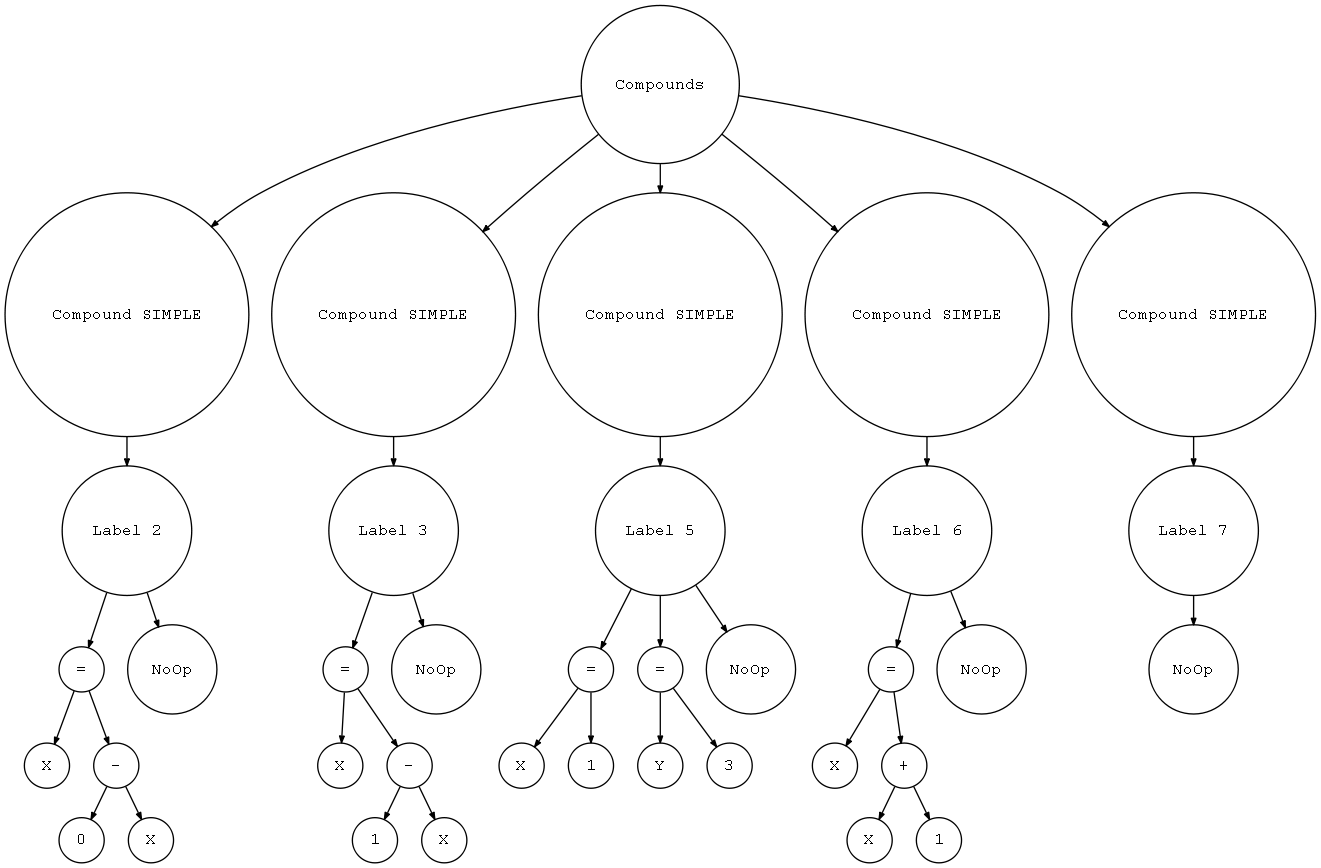
\includegraphics[width=12cm,height=12cm,keepaspectratio]{input/text_source_simple_ast.png}
  \caption{AST du programme text\_source\_simple.txt}
  \label{fig:ast1}
\end{figure}

\begin{figure}[h!]
  \centering
  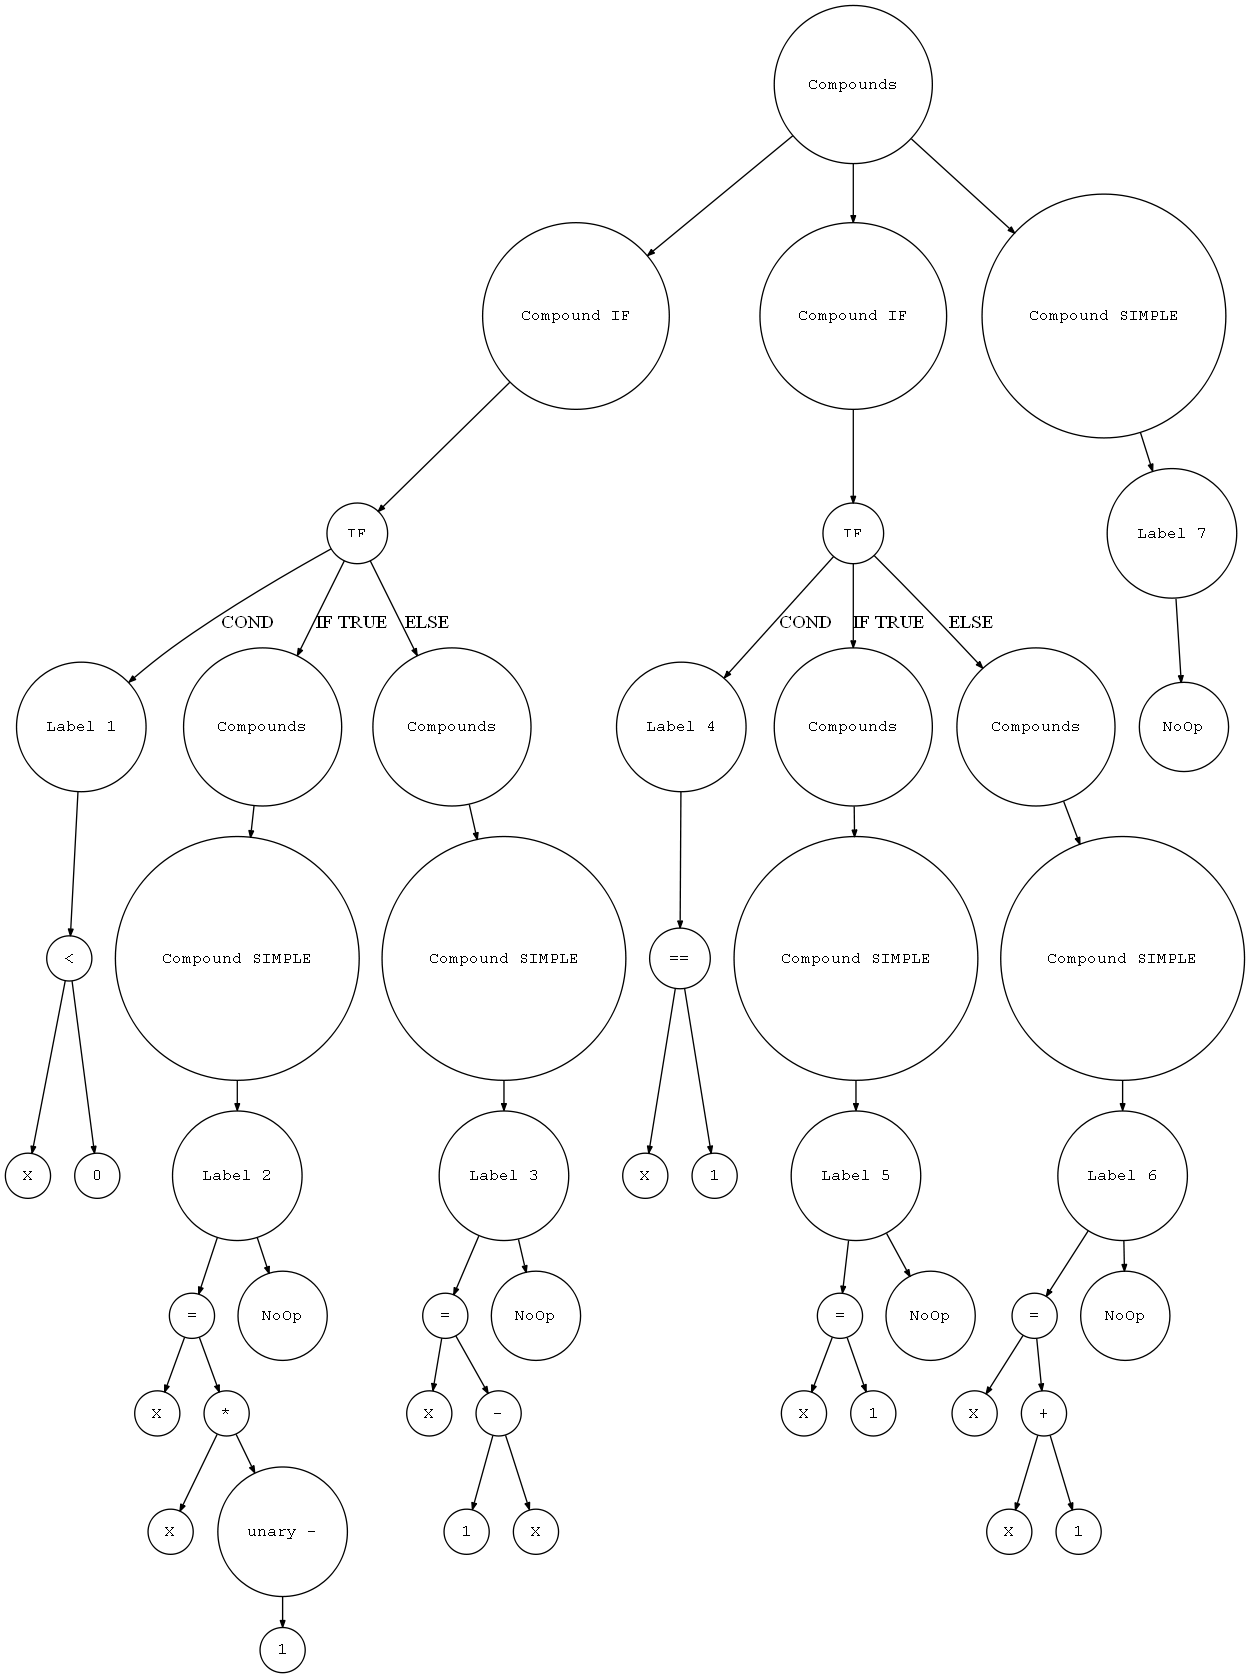
\includegraphics[width=12cm,height=12cm,keepaspectratio]{input/text_source_ast.png}
  \caption{AST du programme text\_source.txt}
  \label{fig:ast2}
\end{figure}

\begin{figure}[h!]
  \centering
  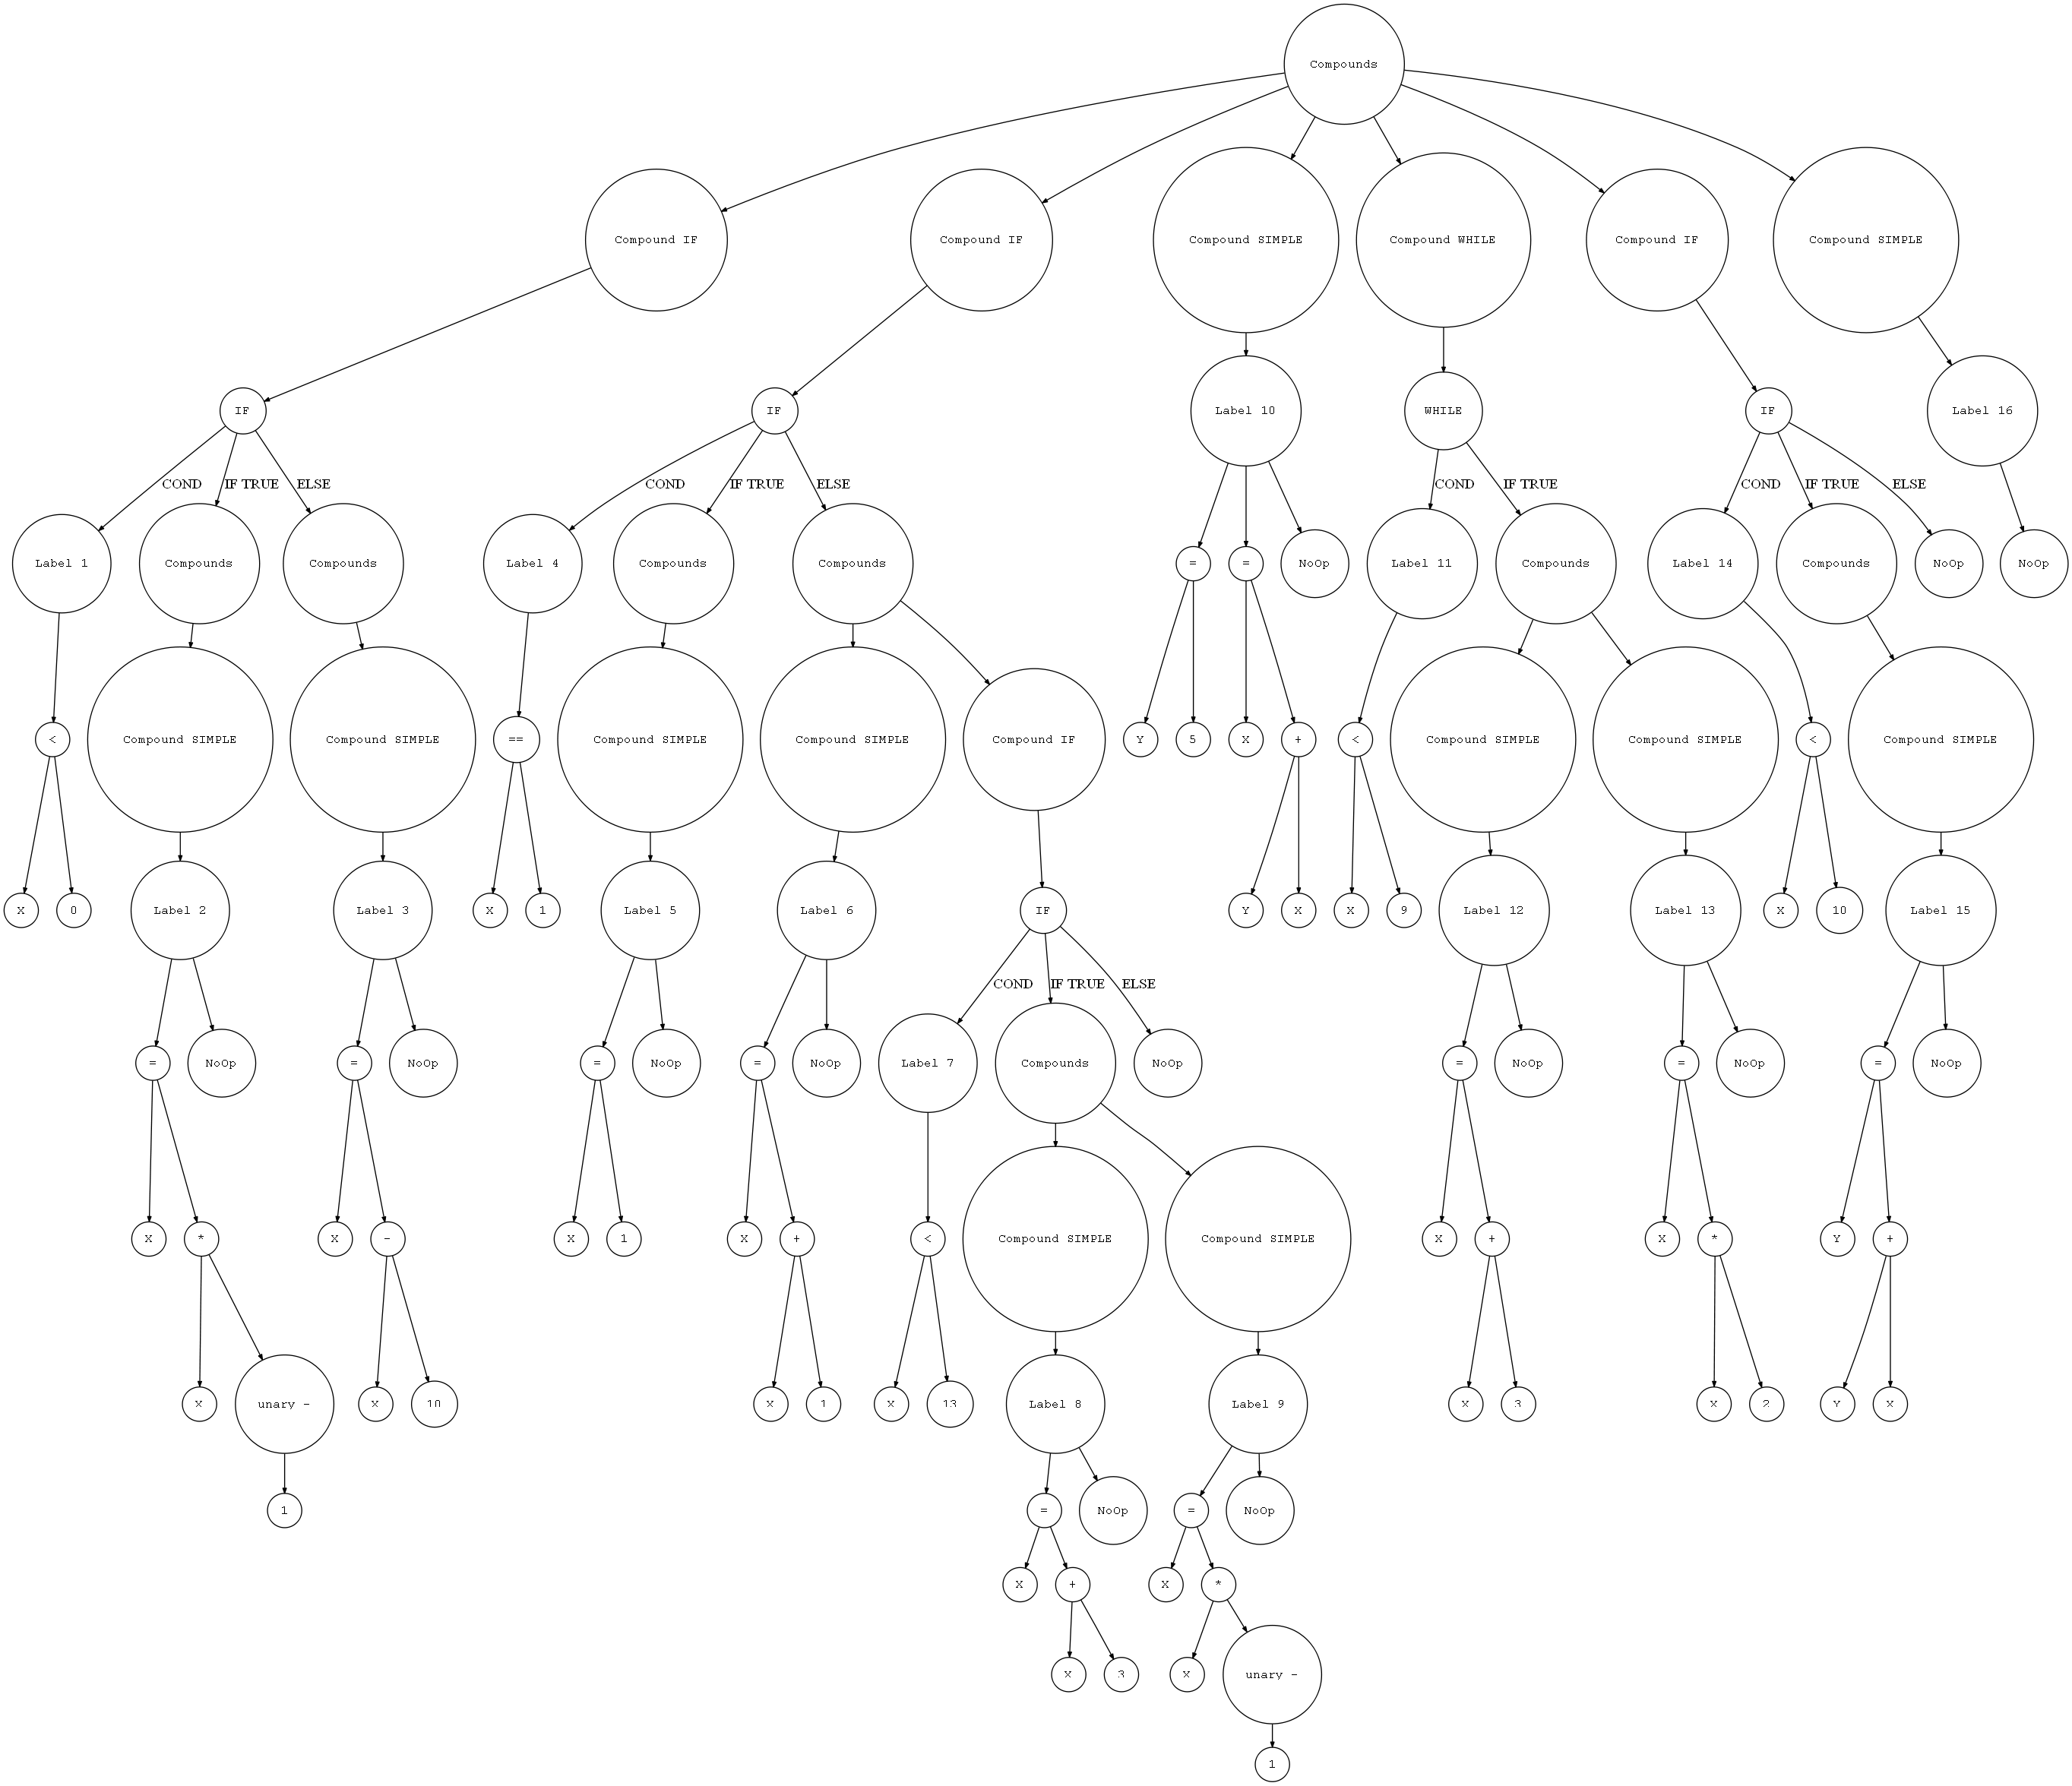
\includegraphics[width=15cm,height=15cm,keepaspectratio]{input/text_source_complique_ast.png}
  \caption{AST du programme text\_source\_complique.txt}
  \label{fig:ast3}
\end{figure}

\begin{figure}[h!]
  \centering
  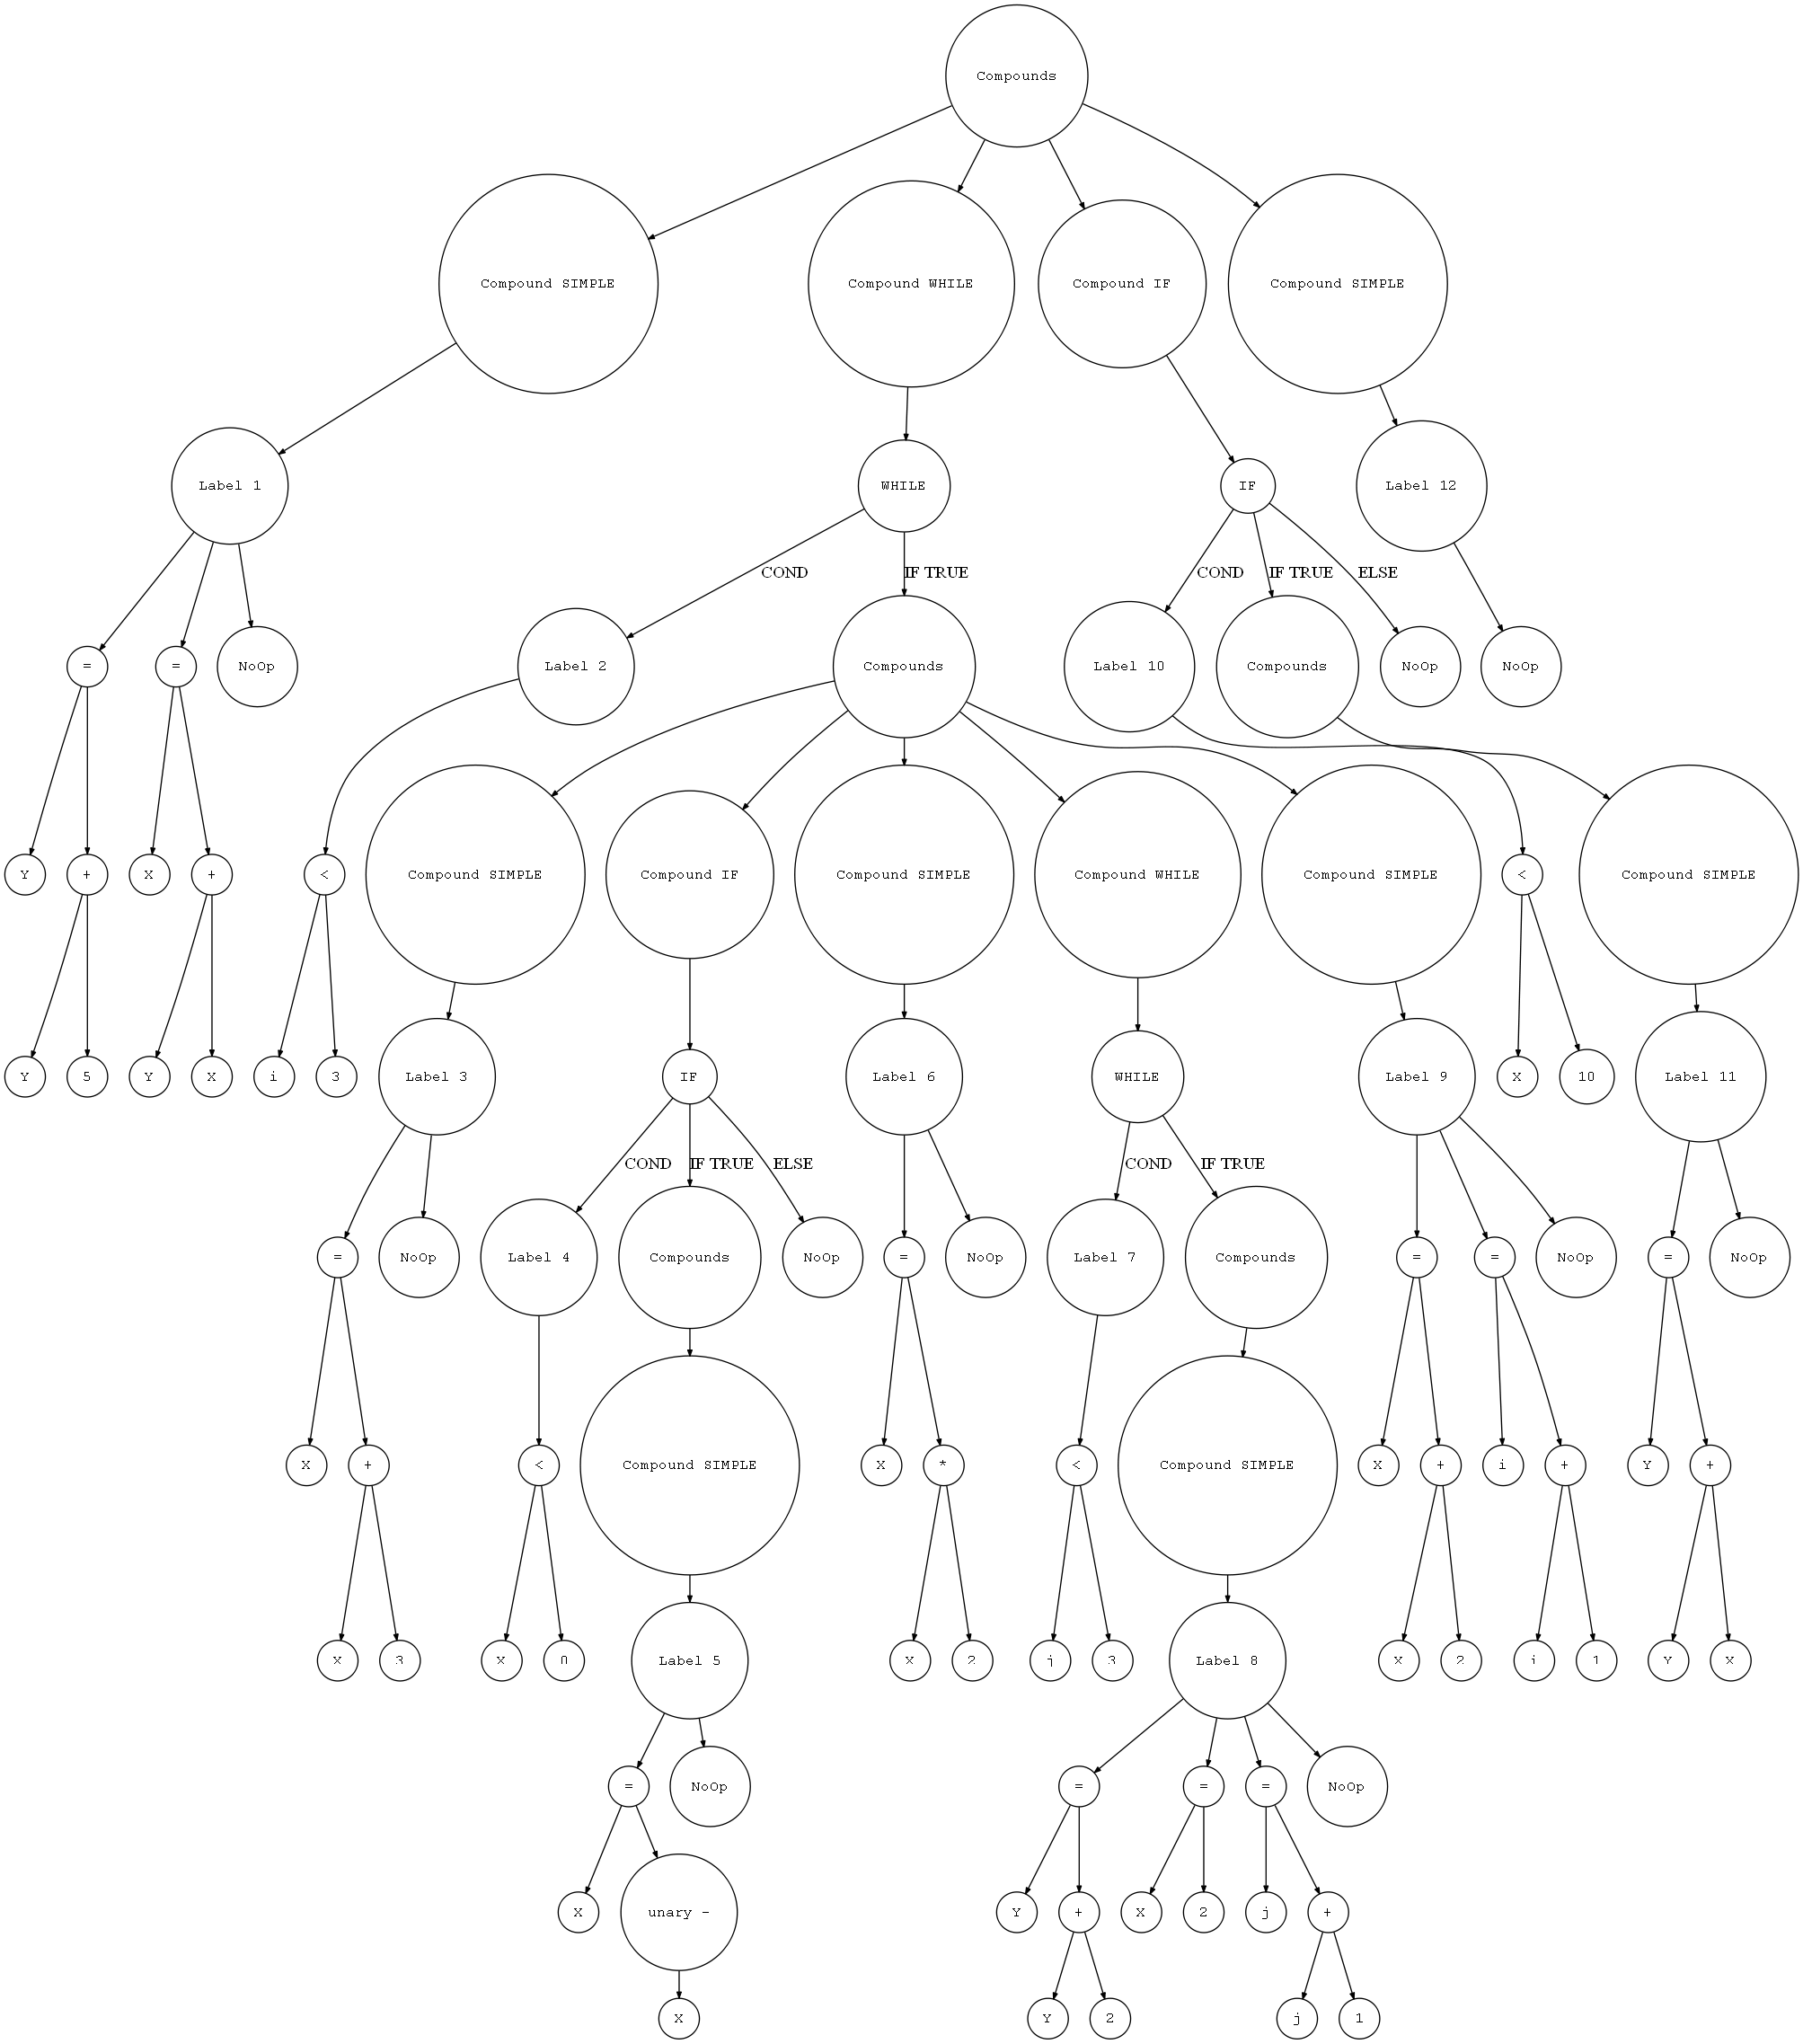
\includegraphics[width=12cm,height=12cm,keepaspectratio]{input/text_source_while_in_a_while_ast.png}
  \caption{AST du programme text\_source\_while\_in\_a\_while.txt}
  \label{fig:ast4}
\end{figure}

\begin{figure}[h!]
  \centering
  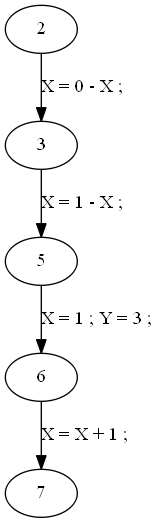
\includegraphics[width=7cm,height=7cm,keepaspectratio]{input/text_source_simple_cfg.png}
  \caption{CFG du programme text\_source\_simple.txt}
  \label{fig:cfg1}
\end{figure}

\begin{figure}[h!]
  \centering
  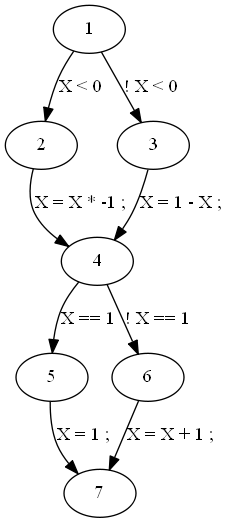
\includegraphics[width=8cm,height=8cm,keepaspectratio]{input/text_source_cfg.png}
  \caption{CFG du programme text\_source.txt}
  \label{fig:cfg2}
\end{figure}

\begin{figure}[h!]
  \centering
  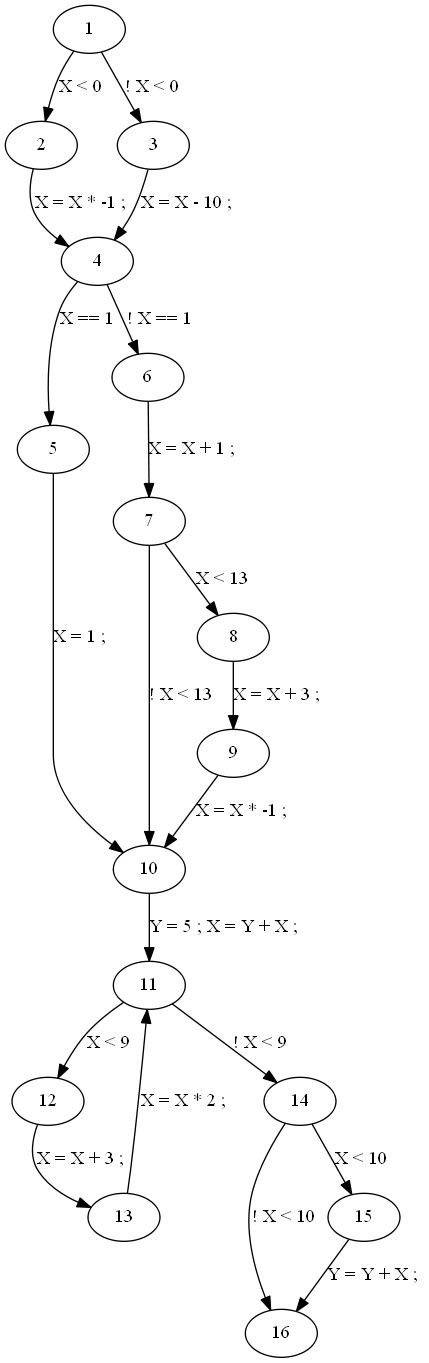
\includegraphics[width=12cm,height=12cm,keepaspectratio]{input/text_source_complique_cfg.png}
  \caption{CFG du programme text\_source\_complique.txt}
  \label{fig:cfg3}
\end{figure}

\begin{figure}[h!]
  \centering
  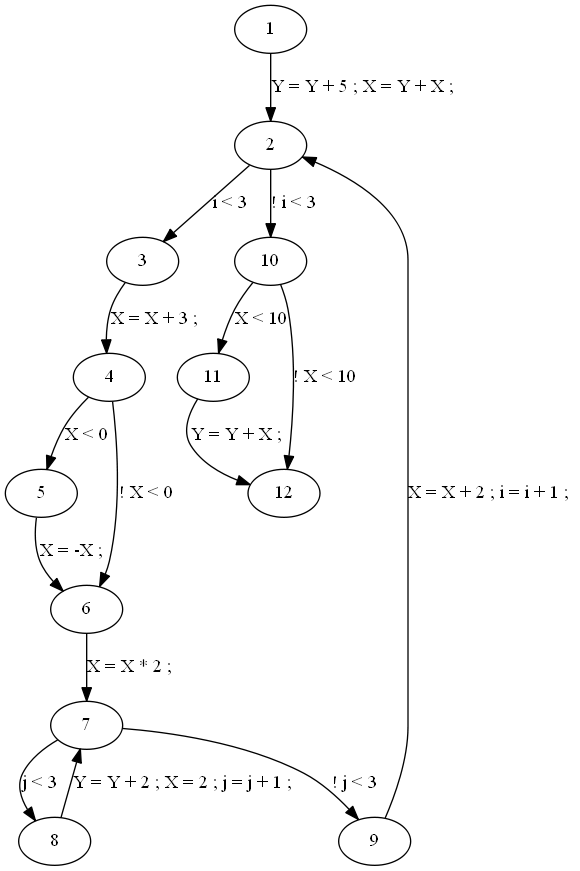
\includegraphics[width=12cm,height=12cm,keepaspectratio]{input/text_source_while_in_a_while_cfg.png}
  \caption{CFG du programme text\_source\_while\_in\_a\_while.txt}
  \label{fig:cfg4}
\end{figure}

\end{document}